\documentclass{standalone}
\usepackage{pgfplots}

\begin{document}
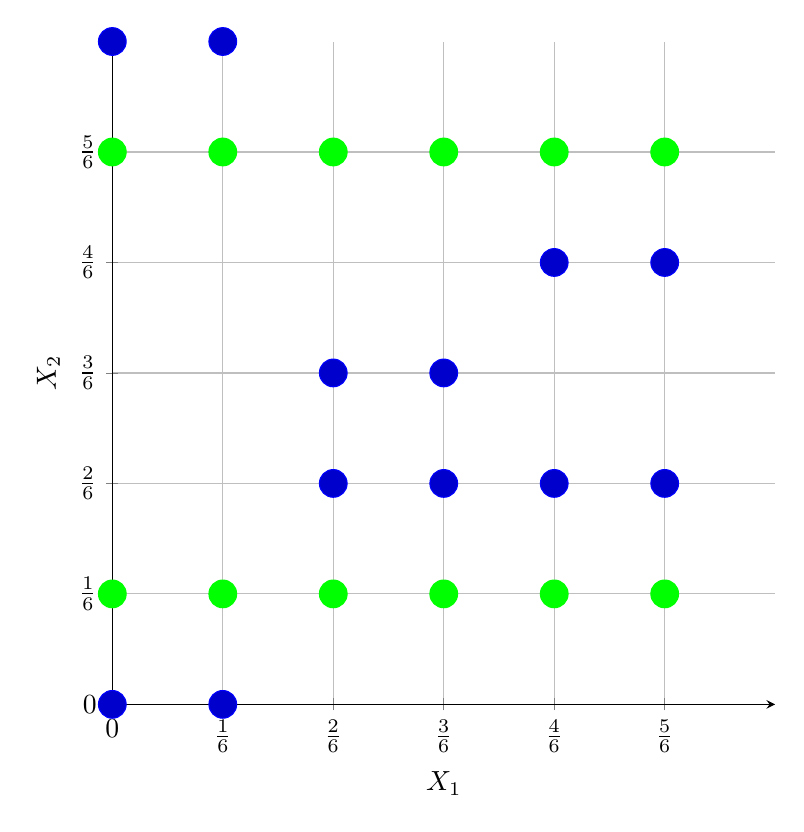
\begin{tikzpicture}
    \begin{axis}[
        axis lines=left,
        xlabel=$X_1$,
        ylabel=$X_2$,
        grid=major,
        xmin=0, xmax=1,
        ymin=0, ymax=1,
        xtick={0,1/6,...,5/6},
        ytick={0,1/6,...,5/6},
        xticklabels={0,$\frac{1}{6}$,$\frac{2}{6}$,$\frac{3}{6}$,$\frac{4}{6}$,$\frac{5}{6}$,$1$},
        yticklabels={0,$\frac{1}{6}$,$\frac{2}{6}$,$\frac{3}{6}$,$\frac{4}{6}$,$\frac{5}{6}$,$1$},
        width=10cm,
        height=10cm,
        every axis plot/.append style={
            mark=*,
            only marks,
            mark size=5pt,
            mark options={solid}
        }
    ]
        % Blue ladder
        \addplot coordinates {
            (0,1) (1/6,1) (2/6,1/2) (3/6,1/2) (4/6,1/3) (5/6,1/3)
            (0,0) (1/6,0) (2/6,1/3) (3/6,1/3) (4/6,2/3) (5/6,2/3)
        };
        
        % Green ladder
        \addplot[green] coordinates {
            (0,5/6) (1/6,5/6) (2/6,5/6) (3/6,5/6) (4/6,5/6) (5/6,5/6)
            (0,1/6) (1/6,1/6) (2/6,1/6) (3/6,1/6) (4/6,1/6) (5/6,1/6)
        };
    \end{axis}
\end{tikzpicture}
\end{document}